\documentclass{beamer}
\usepackage{amsfonts,amsmath,oldgerm}
\usepackage{ragged2e}

\usetheme{sintef}

\newcommand{\testcolor}[1]{\colorbox{#1}{\textcolor{#1}{test}}~\texttt{#1}}

\usefonttheme[onlymath]{serif}

\titlebackground*{assets/background}

\newcommand{\hrefcol}[2]{\textcolor{cyan}{\href{#1}{#2}}}

\title{Aula 00}
\subtitle{2023.1 - SOPA2 - Sistemas Operacionais}
\course{Tecnologia em Análise e Desenvolvimento de Sistemas}
\author{\href{mailto:luizfpq@gmail.com}{Luiz \textbf{Quirino}}}
\IDnumber{luizfpq@gmail.com}



\begin{document}
\maketitle

%\begin{frame}
%
%      Este material é produzido utilizando \LaTeX\, baseado na SINTEF Presentation, disponibilizado sob licenciamento \hrefcol{https://creativecommons.org/licenses/by-nc/4.0/legalcode}{Creative Commons CC BY 4.0}
%
%\vspace{\baselineskip}

%In the following you find a brief introduction on how to use \LaTeX\ and the beamer package to prepare slides, based on the one written by \hrefcol{mailto:federico.zenith@sintef.no}{Federico Zenith} for \hrefcol{https://www.overleaf.com/latex/templates/sintef-presentation/jhbhdffczpnx}{SINTEF Presentation}

% This template is released under \hrefcol{https://creativecommons.org/licenses/by-nc/4.0/legalcode}{Creative Commons CC BY 4.0} license

%\end{frame}

\section{Apresentação}

\begin{frame}{Quem sou eu na fila do pão?}
Formação:
\begin{itemize}
\item Pos-graduação em Gestão de Riscos e CiberSegurança - Focus
\item Sistemas de Informação - UFMS
\item Gestão de Tecnologia da Informação - Unicesumar
\item Técnico em Informática - Centro Paula Souza
\end{itemize}
Atuação:
\begin{itemize}
\item Técnico em Tecnologia da Informação - IFSP
\item Contribuidor OpenSource
\item Desenvolvedor Freelancer
\end{itemize}

\end{frame}

\begin{frame}{Ementa}\justifying
      A disciplina aborda o conjunto de programas usados para gerenciar recursos de
computadores, fornecendo uma interface com o usuário. São trabalhos os fundamentos,
instalação e configuração de sistemas operacionais e aplicativos modernos, gestão de
armazenamento, usuários e processos de software, proporcionando ao estudante habilidade
para selecionar e instalar sistemas operacionais e programas de computador adequados às
necessidades de usuários e empresas, e instalar seu próprio computador de
desenvolvimento.
\end{frame}

\begin{frame}{Objetivo da disciplina}\justifying
      Identificar os fundamentos de sistemas operacionais modernos e a sua importância para
sistemas de informação. Conhecer os mecanismos internos a um sistema operacional.
Selecionar, instalar e configurar sistemas operacionais. Comparar e aplicar diferentes
soluções de sistemas operacionais.
\end{frame}

\begin{frame}[fragile]{Conteúdo Programático}

\begin{itemize}
      \item Fundamentos de Sistemas Operacionais
      \begin{itemize}
            \item História dos sistemas operacionais modernos
            \item Processos, memória, arquivos, entrada/saída e proteção;
            \item Chamadas de sistema;
            \item Estrutura de um SO.
      \end{itemize}
      \item Particionamento de disco e instalação de sistema operacional para Desktop em
      máquina virtual;
      \item Processo de inicialização;
      \item Operações em diretórios e arquivos, Filesystem Hierarchy Standard (FHS);
      \item Comandos para manipulação de arquivos texto;
      \item Permissões e propriedades de arquivos e diretórios;
      \item Programação de scripts shell, parâmetros de entrada, variáveis de ambiente;
    
\end{itemize}
\end{frame}

\begin{frame}[fragile]{Conteúdo Programático}

      \begin{itemize}
            \item Agrupamento e compressão de arquivos;
            \item Sistemas gerenciadores de pacotes;
            \item Gerenciamento de entrada e de saída;
            \item Gerenciamento de pacotes, aplicativos externos à distribuição;
            \item Gerenciamento de processos, escalonamento de processos, interrupções de
            hardware, ciclo de vida de processos, comunicação interprocessos;
            \item Gerenciamento de memória, memória virtual, semáforos, concorrência, threads;
            \item Introdução e prevenção de deadlocks;
            \item Gerenciando usuários, grupos e permissões;
            \item Comandos para analisar partições e sistema de arquivos;
            \item Comandos para analisar o desempenho.
      \end{itemize}
      \end{frame}
      



\section{Planejamento}

\begin{frame}[fragile]{Calendário - Maio}
      \begin{figure}[H]
            \centerline{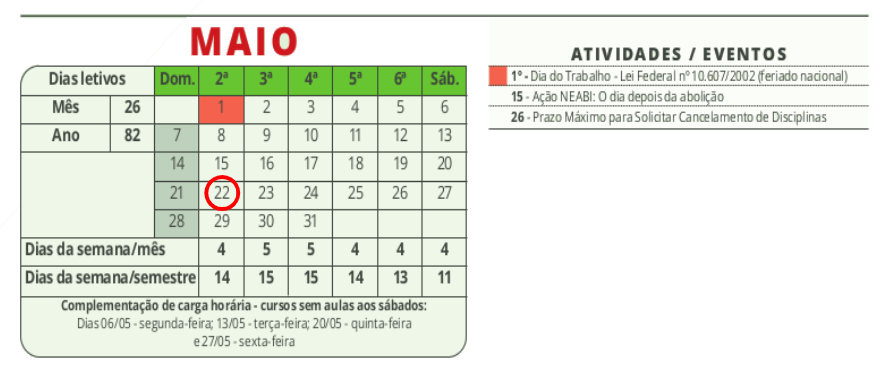
\includegraphics[width=1.1\textwidth]{assets/aula-tads-sopa2-2023-05-22/maio.png}}
            \caption{Calendario academico - maio}
        \end{figure}
\end{frame}

\begin{frame}[fragile]{Calendário - Junho}
      \begin{figure}[H]
            \centerline{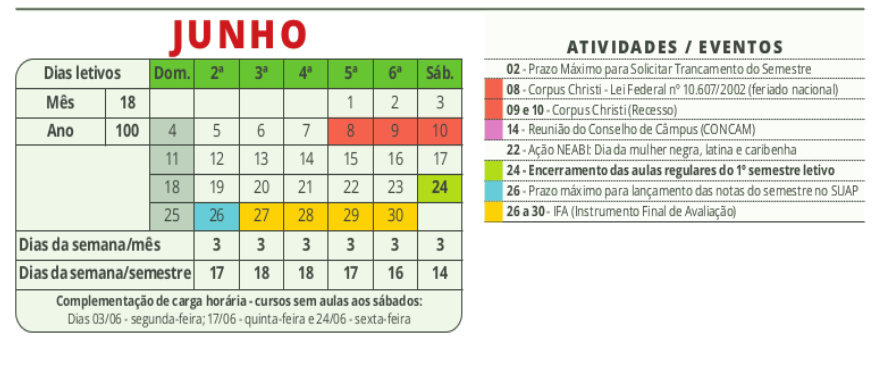
\includegraphics[width=1.1\textwidth]{assets/aula-tads-sopa2-2023-05-22/junho.png}}
            \caption{Calendario academico - junho}
        \end{figure}
\end{frame}

\begin{frame}[fragile]{Calendário - Julho}
      \begin{figure}[H]
            \centerline{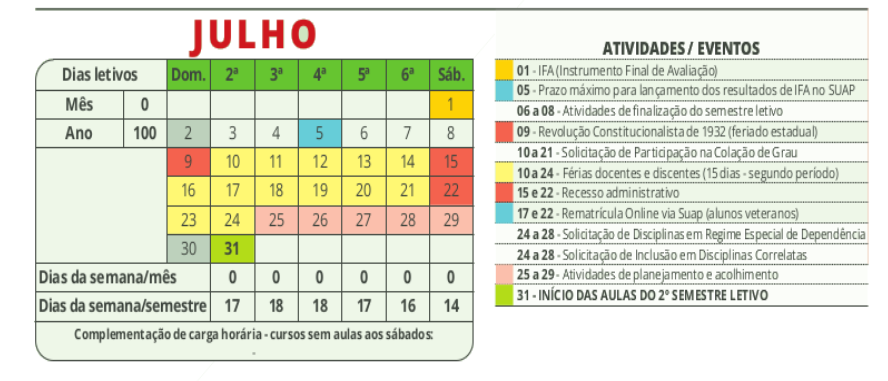
\includegraphics[width=1.1\textwidth]{assets/aula-tads-sopa2-2023-05-22/julho.png}}
            \caption{Calendario academico - julho}
        \end{figure}
\end{frame}

\section{Alinhamento}

\begin{frame}[fragile]{Auto Inscrição Moodle}

      Autoinscrição → Chave: SOPA2@2023.1

      \begin{figure}[H]
            \centerline{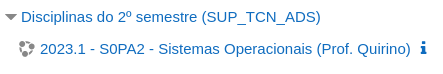
\includegraphics[width=1\textwidth]{assets/aula-tads-sopa2-2023-05-22/moodle.png}}
            
        \end{figure}
\end{frame}

\begin{frame}
\frametitle{Alinhamento}
\begin{itemize}
\item Verificar carga horária a \textbf{repor}
\item Realizar atividades de \textbf{nivelamento} da turma
\item \textbf{Reorganizar} o plano de aulas
\item \textbf{Definir calendário} avaliativo

\end{itemize}
\end{frame}

\backmatter
\end{document}
